\newpage
\section{Analysis of results}

\fmc{Poner en positivo "obtuvimos esto", lo que se podría haber hecho poner como future work...}

\textcolor{gray}{
\begin{itemize}
    \item 1. Tamaño de banco y streams con los que se probó
    \item 2. Para cada tamaño de banco, configuración / maxFilterSizes con los que se probó + versión secuencial
    \item 3. Analisis resultados de forma conjunta de todo.
\end{itemize}
}

\subsection*{E1: Evaluation in a High-Load Stress Scenario}

\subsubsection*{Experimental Variations}

This experiment on the \DPATM system was tested on the two defined synthetic bank databases \smallG and \mediumG. In each case we 
provided streams of different sizes and ratio of anomalous transactions, as detailed in the table \ref{table:stream-sizes}. 

\emph{maxFilterSize}

\begin{table}[H]
    \small 
    \begin{tabular}{|c|c|c|c|c|c|}
    \hline
    \textbf{Bank Database} & \textbf{\# Days} & \textbf{Anomalous Ratio} & \textbf{Stream Size} & \textbf{Regular tx} & \textbf{Anomalous tx} \\ \hline
    \smallG    & 30       & $0.02\ (2\%)$   & 39959       & 39508      & 451 $1\%$    \\ \hline
    \smallG     & 60       & $0.02\ (2\%)$   & 80744       & 79005      & 1739         \\ \hline
    \smallG     & 120      & $0.02\ (2\%)$   & 160750      & 157756     & 2994         \\ \hline
    \mediumG    & 7        & $0.03\ (3\%)$   & 2428286     &            &              \\ \hline
    \mediumG    & 15       & $0.03\ (3\%)$   & 4856573     & 4805920    & 50653        \\ \hline
    \end{tabular}
    \caption{Summary of the different stream sizes generated for each of the bank databases. For each stream we indicate the anomalous ratio, its exact stream size (in the number of transactions), and from it, its number of only regular and only anomalous transactions}
    \label{table:stream-sizes}
\end{table}

In addition, appart from providing different streams 


\textbf{ONLY CHECKS in these experiments}

For different core variations, we are going to try different combinations of the system in terms
of the number of the maximum number of cards per filter, that consequently will produce an inverse variation in the number of filters of the system.

\subsubsection*{\smallG}
    
\begin{table}[H]
    \renewcommand{\arraystretch}{1.5} % control row height
    \centering
    \begin{tabular}{|c|c|}
    \hline
    \# cards per filter & \# filters \\ \hline
    2000   &   1     \\ \hline
    1000   &   2     \\ \hline
    400 &   5     \\ \hline
    200  &   10     \\ \hline
    100 &   20    \\ \hline
    50  &   40    \\ \hline
    20  &   100    \\ \hline
    10  &   200    \\ \hline
    4  &   500    \\ \hline
    2  &   1000    \\ \hline
    1  &   2000    \\ \hline
    \end{tabular}
\end{table}
    
\begin{itemize}
    \item \# of times / runs each job $=10$.
    \item Maximum RAM limited to 16GB.
    \item Run for 1c, 2c, 4c, 8c and 16c.
\end{itemize}

\paragraph{Results Analysis\\}

\begin{itemize}
    \item Better behavior for a number of filters: 5,10,20 (not lowest, not really high)
    \item How the number of cores influences in the improve of the behavior
\end{itemize}

\paragraph{Comparison of behavior depending on the number of filters}

\paragraph{Exec time plots - for a core number - different stream sizes\\}
\newpage
\begin{figure}[H]
    \centering
    % Temporarily adjust margins for wider content
    \makebox[\textwidth][c]{%
        \begin{minipage}{0.5\textwidth}
            \centering
            \includegraphics[scale=0.5]{images/4-Experiments/E1-NRT/30-0.02/16c/execTime.png}
            \caption*{30-0.02}
        \end{minipage}
        \hspace{0.1\textwidth}
        \begin{minipage}{0.5\textwidth}
            \centering
            \includegraphics[scale=0.5]{images/4-Experiments/E1-NRT/60-0.02/16c/execTime.png}
            \caption*{60-0.02}
        \end{minipage}
    }
    
    \vspace{0.5cm} % Vertical space between rows

    \makebox[\textwidth][c]{%
        \begin{minipage}{0.5\textwidth}
            \centering
            \includegraphics[scale=0.5]{images/4-Experiments/E1-NRT/120-0.02/16c/execTime.png}
            \caption*{120-0.02}
        \end{minipage}
    }

    \caption{Execution Time Plots for 16c}
    \label{img:exps-small-execTime-16c}
\end{figure}


\paragraph{MRT plots - for a core number 16 - different stream sizes\\}
\newpage

\begin{figure}[H]
    \centering
    % Temporarily adjust margins for wider content
    \makebox[\textwidth][c]{%
        \begin{minipage}{0.5\textwidth}
            \centering
            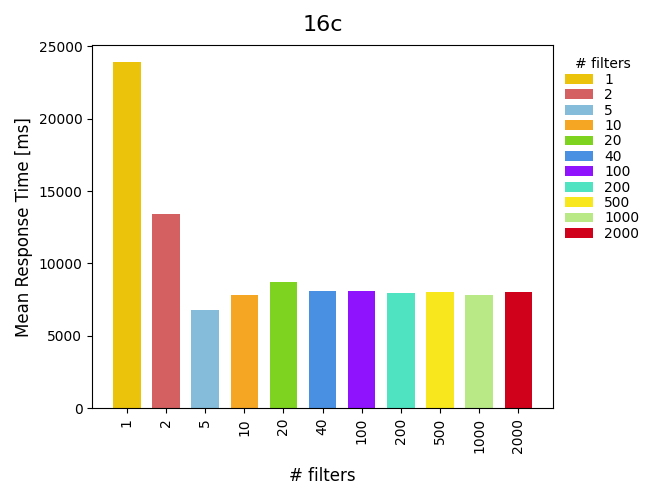
\includegraphics[scale=0.5]{images/4-Experiments/E1-NRT/30-0.02/16c/mrt.png}
            \caption*{30-0.02}
        \end{minipage}
        \hspace{0.1\textwidth}
        \begin{minipage}{0.5\textwidth}
            \centering
            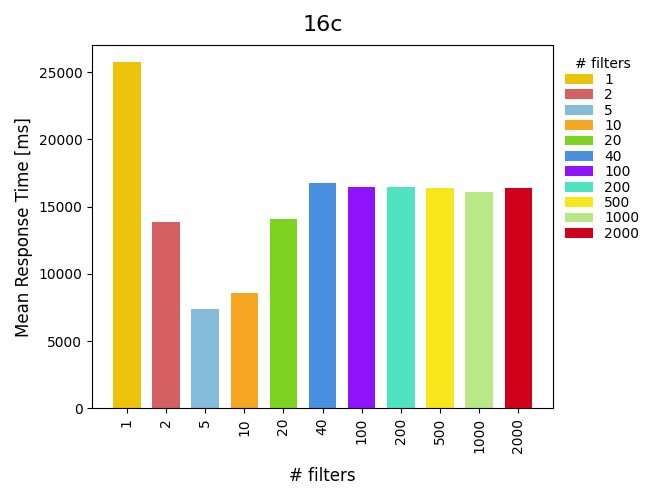
\includegraphics[scale=0.5]{images/4-Experiments/E1-NRT/60-0.02/16c/mrt.png}
            \caption*{60-0.02}
        \end{minipage}
    }
    
    \vspace{0.5cm} % Vertical space between rows

    \makebox[\textwidth][c]{%
        \begin{minipage}{0.5\textwidth}
            \centering
            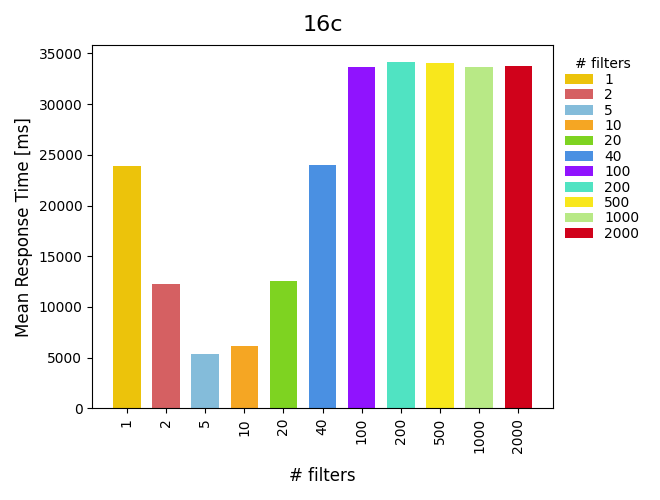
\includegraphics[scale=0.5]{images/4-Experiments/E1-NRT/120-0.02/16c/mrt.png}
            \caption*{120-0.02}
        \end{minipage}
    }

    \caption{MRT Plots for 16c}
    \label{img:exps-small-mrt-16c}
\end{figure}

\paragraph{Trace and response time trace for 16c and big stream\\}
\newpage

\begin{figure}[H]
    \centering
    % Subfigures arranged vertically
    \begin{subfigure}[b]{\textwidth}
        \centering
        \includegraphics[scale=0.5]{images/4-Experiments/E1-NRT/30-0.02/16c/traces-response-time-reduced.png}
        \caption{30-0.02}
    \end{subfigure}
    
    \vspace{0.5cm} % Vertical space between subfigures
    \begin{subfigure}[b]{\textwidth}
        \centering
        \includegraphics[scale=0.5]{images/4-Experiments/E1-NRT/60-0.02/16c/traces-response-time-reduced.png}
        \caption{60-0.02}
    \end{subfigure}
    
    \vspace{0.5cm} % Vertical space between subfigures
    \begin{subfigure}[b]{\textwidth}
        \centering
        \includegraphics[scale=0.5]{images/4-Experiments/E1-NRT/120-0.02/16c/traces-response-time-reduced.png}
        \caption{120-0.02}
    \end{subfigure}

    \caption{Response Time Traces for 16c}
    \label{img:exps-small-responsetimetraces-16c}
\end{figure}

\paragraph{Trace and response time trace for 16c and big stream\\}

\begin{figure}[H]
    \centering
    % Subfigures arranged vertically
    \begin{subfigure}[b]{\textwidth}
        \centering
        \includegraphics[scale=0.5]{images/4-Experiments/E1-NRT/30-0.02/16c/traces.png}
        \caption{30-0.02}
    \end{subfigure}
    
    \vspace{0.5cm} % Vertical space between subfigures
    \begin{subfigure}[b]{\textwidth}
        \centering
        \includegraphics[scale=0.5]{images/4-Experiments/E1-NRT/60-0.02/16c/traces.png}
        \caption{60-0.02}
    \end{subfigure}
    
    \vspace{0.5cm} % Vertical space between subfigures
    \begin{subfigure}[b]{\textwidth}
        \centering
        \includegraphics[scale=0.5]{images/4-Experiments/E1-NRT/120-0.02/16c/traces.png}
        \caption{120-0.02}
    \end{subfigure}

    \caption{Results Traces for 16c}
    \label{img:exps-small-traces-16c}
\end{figure}

\begin{figure}[H]
    \centering
    % Temporarily adjust margins for wider content
    \hspace*{-3cm} % Move content to the left by 2 cm (adjust as needed)
    \begin{minipage}{0.5\textwidth}
        \centering
        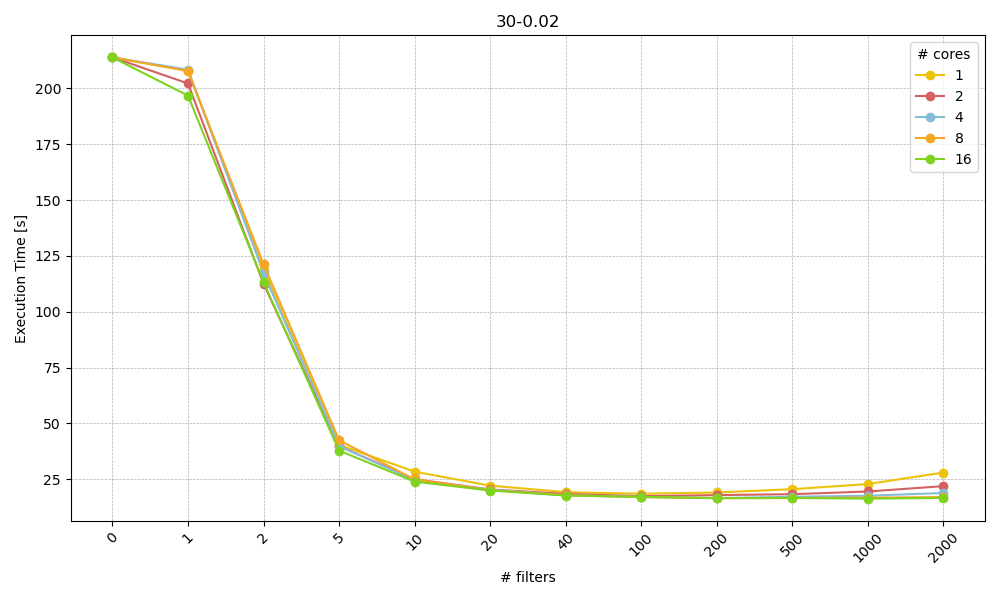
\includegraphics[scale=0.4]{images/4-Experiments/E1-NRT/120-0.02/combined/execTime-1.png}
        \caption*{}
    \end{minipage}
    \hspace{0.16\textwidth}
    \begin{minipage}{0.5\textwidth}
        \centering
        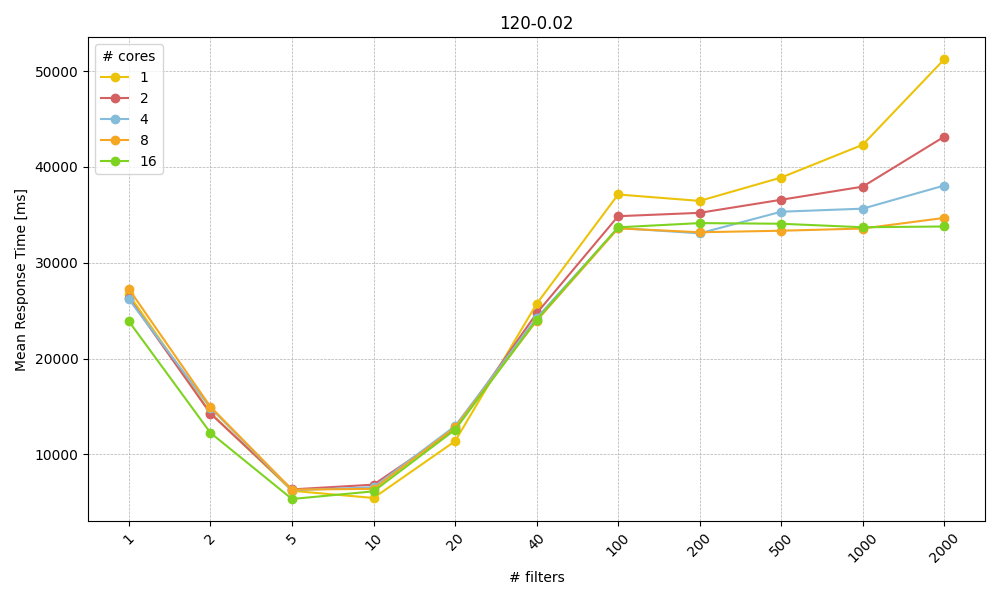
\includegraphics[scale=0.4]{images/4-Experiments/E1-NRT/120-0.02/combined/mrt-1.png}
        \caption*{}
    \end{minipage}
    
    \vspace{0.5cm} % Vertical space between rows

    \hspace*{-3cm} % Move content to the left for the second row
    \begin{minipage}{0.5\textwidth}
        \centering
        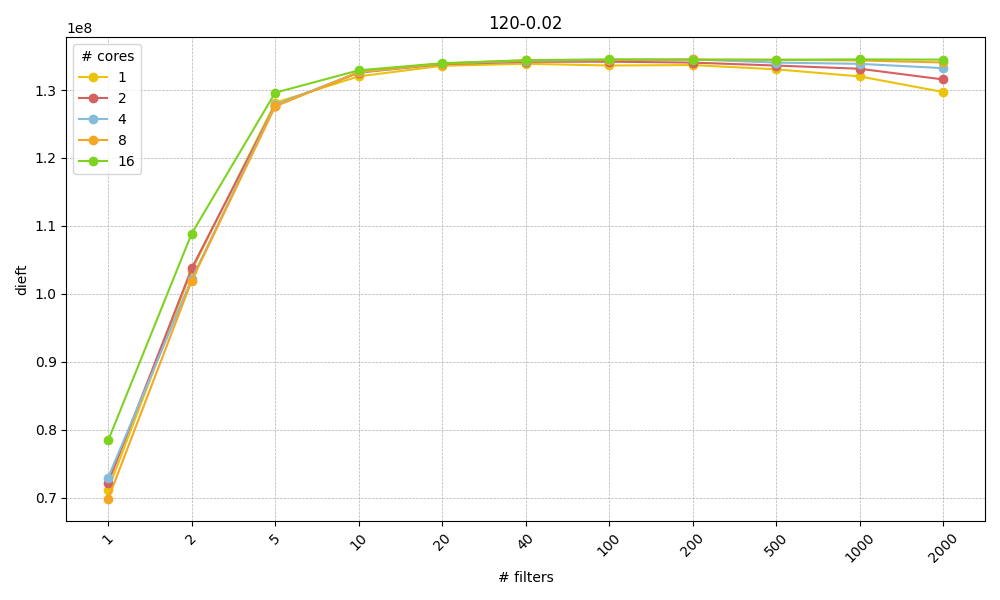
\includegraphics[scale=0.4]{images/4-Experiments/E1-NRT/120-0.02/combined/dieft-1.png}
        \caption*{}
    \end{minipage}
    \hspace{0.16\textwidth}
    \begin{minipage}{0.5\textwidth}
        \centering
        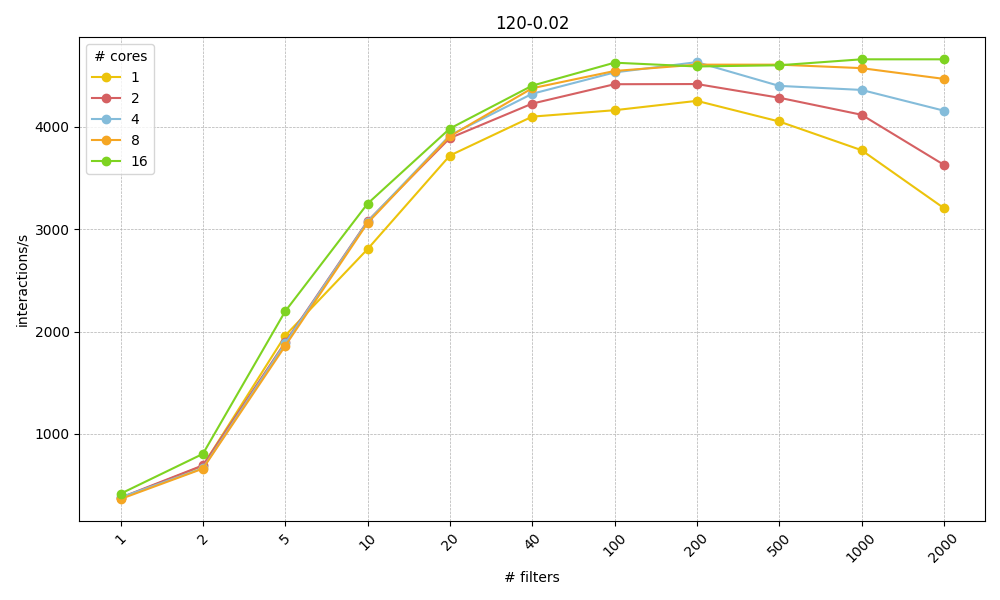
\includegraphics[scale=0.4]{images/4-Experiments/E1-NRT/120-0.02/combined/interactions-1.png}
        \caption*{}
    \end{minipage}

    \caption{Combined cores and filters variation plots for big stream: 120-0.02}
    \label{img:exps-small-120-combined}
\end{figure}

\fmc{Decidir qué poner, redactar bien las interpretaciones}
Interpretation:
\begin{itemize}
     \item \ref{img:exps-small-responsetimetraces-16c} For the smallest stream size 
     the response time of 1f (sequential) is always higher than when using more filters. However for larger stream sizes this is not the case, since from a certain point the response time tends to be higher, showing an accumulation... overhead?
     \item Conclusions: less filters maintain constant the RT (especially better for large stream sizes / where we have longer periods of high loaded scenarios). More filters however tend to get increased their response time, accumulating. In the middle, 5, 10 and 20 filters tend to be the best tradeoff between low and constant response time and low execution time / time needed to process all the input stream.
     \item The continuous behavior is better while increasing the number of filters for all the number of cores variations in terms of the \texttt{dief@t} metric, this can be seen in the \texttt{dief@t} plot in the Figure \ref{img:exps-small-120-combined}. It can also be seen in the traces plot in Figure \ref{img:exps-small-traces-16c} which shows the result traces in the case of the variations run with 16c. Note the slight degradation of the \texttt{dief@t} in the variations with the highest number of filters (from 100 and on, but specially on the cases with 1000 and 2000 filters), in the variations run with low number of cores: Figure \ref{img:exps-small-120-combined}.
     \item However measuring the behavior in terms of the execution time (total needed time to process the full stream input) and the mean response time and response time traces, we can see that for a same core configuration (e.g. 16 cores), the total execution time (time to process all the stream input) is larger for the approaches with less filters, tending to decrease. However the behavior in terms of the response time is different: the best is observed for a number of filters in the range of 5-10 filters. From that point and on the mean response time tends to degrade when increasing the number filters, especially for bigger stream sizes. Even larger than the lowest number of filters version (close to a sequential version) in these cases. This can be due to an overhead on the number of goroutines utilized and the overhead in the communication of the pipeline that this is causing.
\end{itemize}


\paragraph{Comparison of behavior depending on the number of cores}
\begin{itemize}
    \item More cores help to improve the behavior, especially for the variants with large number of filters (expected).
\end{itemize}

\begin{figure}[H]
    \centering
    % Temporarily adjust margins for wider content
    \makebox[\textwidth][c]{%
        \begin{minipage}{0.5\textwidth}
            \centering
            \includegraphics[scale=0.6]{images/4-Experiments/E1-NRT/120-0.02/fixedfilters/5f/execTime.png}
            \caption*{}
        \end{minipage}
        \hspace{0.08\textwidth}
        \begin{minipage}{0.5\textwidth}
            \centering
            \includegraphics[scale=0.6]{images/4-Experiments/E1-NRT/120-0.02/fixedfilters/20f/execTime.png}
            \caption*{}
        \end{minipage}
    }
    
    \vspace{0.5cm} % Vertical space between rows

    \makebox[\textwidth][c]{%
        \begin{minipage}{0.5\textwidth}
            \centering
            \includegraphics[scale=0.6]{images/4-Experiments/E1-NRT/120-0.02/fixedfilters/100f/execTime.png}
            \caption*{}
        \end{minipage}
        \hspace{0.08\textwidth}
        \begin{minipage}{0.5\textwidth}
            \centering
            \includegraphics[scale=0.6]{images/4-Experiments/E1-NRT/120-0.02/fixedfilters/1000f/execTime.png}
            \caption*{}
        \end{minipage}
    }

    \caption{Execution Time Fixed filters plots for stream 120-0.02}
    \label{img:exps-read-input-variants}
\end{figure}

\begin{figure}[H]
    \centering
    % Temporarily adjust margins for wider content
    \makebox[\textwidth][c]{%
        \begin{minipage}{0.5\textwidth}
            \centering
            \includegraphics[scale=0.6]{images/4-Experiments/E1-NRT/120-0.02/fixedfilters/5f/mrt.png}
            \caption*{}
        \end{minipage}
        \hspace{0.08\textwidth}
        \begin{minipage}{0.5\textwidth}
            \centering
            \includegraphics[scale=0.6]{images/4-Experiments/E1-NRT/120-0.02/fixedfilters/20f/mrt.png}
            \caption*{}
        \end{minipage}
    }
    
    \vspace{0.5cm} % Vertical space between rows

    \makebox[\textwidth][c]{%
        \begin{minipage}{0.5\textwidth}
            \centering
            \includegraphics[scale=0.6]{images/4-Experiments/E1-NRT/120-0.02/fixedfilters/100f/mrt.png}
            \caption*{}
        \end{minipage}
        \hspace{0.08\textwidth}
        \begin{minipage}{0.5\textwidth}
            \centering
            \includegraphics[scale=0.6]{images/4-Experiments/E1-NRT/120-0.02/fixedfilters/1000f/mrt.png}
            \caption*{}
        \end{minipage}
    }

    \caption{Mean Response Time Fixed filters plots for stream 120-0.02}
    \label{img:exps-read-input-variants}
\end{figure}

\subsubsection{Medium Bank Size}
  
\textcolor{red}{For these experiments, to generate the stream of tx, we needed to simplify this process in order to be able to generate a stream in a feasible amount of time. In particular we used the simplifed version of the \texttt{txGenerator.py}: \texttt{txGenerator-simplified.py} $\rightarrow$ with a random ATM-subset instead of a closest to client ATM-subset. Also variation on the transaction distribution times.}
  

- Initial filter configuration setups:
\begin{table}[H]
\renewcommand{\arraystretch}{1.5} % control row height
\centering
\begin{tabular}{|c|c|}
\hline
\# cards per filter & \# filters \\ \hline
500000   &   1     \\ \hline
100000   &   5     \\ \hline
50000 &   10     \\ \hline
5000  &   100     \\ \hline
2000 &   250    \\ \hline
1000  &   500    \\ \hline
500  &   1000    \\ \hline
250  &   2000    \\ \hline
100  &   5000    \\ \hline
50  &   10000    \\ \hline
10  &   50000    \\ \hline
\end{tabular}
\end{table}

Run with:
\begin{itemize}
    \item 16GB RAM
    \item x1 run each job
\end{itemize}

\begin{itemize}
    \item x: Run and plots done.
    \item " ": Not run.
    \item outMem: out of memory error.
\end{itemize}

\textbf{Stream - 7 Days}
\begin{table}[H]
  \begin{tabular}{|c|c|c|c|c|c|c|c|c|c|c|c|}
  \hline
  \#cores & 1f & 5f & 10f & 100f & 250f & 500f & 1000f & 2000f & 5000f & 10000f & 50000f \\ \hline
  1       &   & x & x & x & x & x & x & x & x & x &        \\ \hline
  2       &   & x & x & x & x & x & x & x & x & x &        \\ \hline
  4       &   & x & x & x & x & x & x & x & x & x &        \\ \hline
  8       &   & x & x & x & x & x & x & x & x & x &        \\ \hline
  16      & x & x & x & x & x & x & x & x & x & x & outMem \\ \hline
  \end{tabular}
\end{table}

Plots:
\begin{itemize}
    \item FixedCores: OK
    \item FixedFilters: OK
    \item Combined: TODO, increase RAM memory to do it, higher than 64GB...
\end{itemize}



\textbf{Stream - 15 Days}
\begin{table}[H]
  \begin{tabular}{|c|c|c|c|c|c|c|c|c|c|c|c|}
  \hline
  \#cores & 1f & 5f & 10f & 100f & 250f & 500f & 1000f & 2000f & 5000f & 10000f & 50000f \\ \hline
  1       &   & x & x & x & x & x & x & x & x & x &        \\ \hline
  2       &   & x & x & x & x & x & x & x & x & x &        \\ \hline
  4       &   & x & x & x & x & x & x & x & x & x &       \\ \hline
  8       & x & x & x & x & x & x & x & x & x & x &        \\ \hline
  16      & x & x & x & x & x & x & x & x & x & x & outMem \\ \hline
  \end{tabular}
\end{table}

Plots:
\begin{itemize}
    \item FixedCores: TODO
    \item FixedFilters: TODO
    \item Combined: TODO
\end{itemize}
  

Based on the results seen (it seems that a really great number of filters is not beneficial), we want to see what happens with a combination of a lower number of filters (like in the experiments for the small bank database):


\begin{table}[H]
    \renewcommand{\arraystretch}{1.5} % control row height
    \centering
    \begin{tabular}{|c|c|}
    \hline
    \# cards per filter & \# filters \\ \hline
    2000   &   1     \\ \hline
    1000   &   2     \\ \hline
    400 &   5     \\ \hline
    200  &   10     \\ \hline
    100 &   20    \\ \hline
    50  &   40    \\ \hline
    20  &   100    \\ \hline
    10  &   200    \\ \hline
    4  &   500    \\ \hline
    2  &   1000    \\ \hline
    1  &   2000    \\ \hline
    \end{tabular}
\end{table}


\textbf{Stream - 7 Days}
\begin{table}[H]
    \begin{tabular}{|c|c|c|c|}
    \hline
    \#cores & 20f & 40f & 200f \\ \hline
    1       &     &     &      \\ \hline
    2       &     &     &      \\ \hline
    4       &     &     &      \\ \hline
    8       &     &     &      \\ \hline
    16      &     &     &      \\ \hline
    \end{tabular}
\end{table}

Results: DONE

Plots:
\begin{itemize}
    \item FixedCores: Running
    \item FixedFilters: Running
    \item Combined: TODO, increase RAM memory to do it, higher than 64GB...
\end{itemize}


\textbf{Stream - 15 Days}
\begin{table}[H]
    \begin{tabular}{|c|c|c|c|c|}
    \hline
    \#cores & 2f & 20f & 40f & 200f \\ \hline
    1       &    &     &     &      \\ \hline
    2       &    &     &     &      \\ \hline
    4       &    &     &     &      \\ \hline
    8       &    &     &     &      \\ \hline
    16      &    &     &     &      \\ \hline
    \end{tabular}
\end{table}

Results: Done

Plots:
\begin{itemize}
    \item FixedCores: TODO
    \item FixedFilters: TODO
    \item Combined: TODO, increase RAM memory to do it, higher than 64GB...
\end{itemize}

\subsection*{E2: Evaluation in a Real-World Stress Scenario}

\fmc{TODO: Describir y poner resultados}
For the experiments perform The real-case scenario and the high loaded test scenario. In the first case, the interactions, although read by a file of artificial simulated interactions, are provided to the pipeline data stream in such a way that they simulate their actual arrival time to the system, with the corresponding time separation between them. In the second case, the interactions are provided just one after the other as fast as possible as they are read.\\

\fmc{TODO: Describir la configuración/entorno donde corrimos los experimentos - maquinas del cluster, con + o - RAM... poner sus características}